\documentclass{beamer}
\usepackage{ifpdf}
\usepackage{grffile}
\usepackage{epsfig} % This package formats figures.
\usepackage{psfrag} % This package formats figures.
\usepackage{amsmath} % This is a package for math features.
\usepackage{amsfonts} % This is a package for math features.
\usepackage{amssymb} % This is a package for math features.
\usepackage{graphicx}
\usepackage{epstopdf}


\usetheme{CambridgeUS}
\begin{document}

\title[Probabilistic Networks]{Networks with Probabilistic Failures}
\subtitle[Probabilistically Scoring Message Priorities]{Scoring Message Priorities in Switched Networks with Probabilistic Failures}
\author[Shubham]{Shubham Goel}
\institute[IITB]{
  Indian Institute of Technology, Bombay\\[1ex]
}
\date[Summer 2016]{Summer 2016}

\begin{frame}[plain]
  \titlepage
\end{frame}

\begin{frame}
\frametitle{Introduction}
	% A picture of a network/messages\\
	\begin{columns}
	\column{0.45\textwidth}
	\begin{figure}
	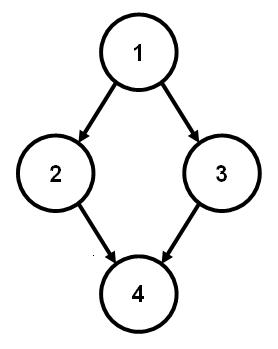
\includegraphics[scale=0.3]{media/digraph2.jpg}
	\caption{Network as a DiGraph}
	\end{figure}
	\column{0.55\textwidth}
	\begin{description}
	\item[G] - A directed graph
	\item[M] - A set of messages (source,target)
	\item[t] - A global timeout
	\end{description}
	\end{columns}
	\vspace*{20pt}
	Hardware Limitation : Only 1 message can be sent per link per time unit
\end{frame}

\begin{frame}
\frametitle{Initial Work}
	\framesubtitle{Time-Triggered (TT) schedules}

	\vspace*{-8pt}

	\begin{columns}
	\column{0.5\textwidth}
	\begin{figure}
	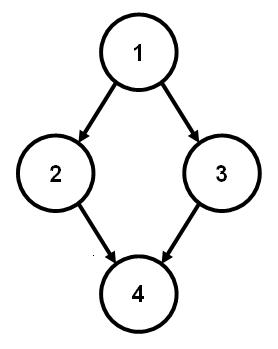
\includegraphics[scale=0.4]{media/digraph2.jpg}
	\caption{Network as a DiGraph}
	\end{figure}

	\column{0.5\textwidth}

	\begin{table}
	\begin{tabular}{c | c | c}
	Message & Source & Target\\
	\hline \hline
	m0 & v1 & v2\\ 
	m1 & v1 & v4
	\end{tabular}
	\caption{Messages}
	\end{table}

	\vspace*{-15pt}

	\begin{table}
	\begin{tabular}{c | c | c}
	Message & Edge & Time\\
	\hline \hline
	m0 & (1-2) & 0\\ 
	m1 & (1-2) & 1\\
	m1 & (2-4) & 2
	\end{tabular}
	\caption{A Time-Triggered Schedule}
	\end{table}
	\end{columns}


	\pause
	\color{red}

	\vspace*{-15pt}
	\begin{center}
	TT scheduling assumes that the network is fixed\\
	However, in practice, networks are faulty (discussed later)
	\end{center}
\end{frame}

\begin{frame}
\frametitle{Previous Paper - An Adverserial Approach}
	\begin{itemize}
	\item Time-Triggered Schedules
	\item Simple Error Recovery Protocol - forward message on some other edge
	\item $(k,l)-resistance$ : If at most $k$ crashes occur, at least $l$ messages arrive\\[3ex]
	\end{itemize}
	\hspace*{20pt}$ crash $ : A link goes down permanently\\[3ex]
	\color{blue}
	In contrast to this, we study networks where the occurence of faults is probablistic. You will find a more detailed specification ahead.
\end{frame}

\begin{frame}
\frametitle{Handling New Faults}
	\begin{itemize}
	\item Edge faults
	\begin{itemize}
		\item Permanent Crashes 
		\item Temporary Crashes
	\end{itemize}
	\item Message faults
	\begin{itemize}
		\item Message Losses
		\item Message Delays\\[2ex]
	\end{itemize}
	\end{itemize}
	\pause
	\begin{center}
	\color{red}
	Things become messy with Time-Triggered Schedules.\\We move to a cleaner notion of message forwarding.
	\end{center}
\end{frame}


% \begin{frame}
% \frametitle{Example}



% \end{frame}


\begin{frame}
\frametitle{Message Forwarding}
	\framesubtitle{Components}
	% \begin{enumerate}
	\begin{block}{Paths}
	For each message $ m\in M $, specify the possible paths that can be taken by $ m $
	\end{block}

	\begin{block}{Priority Scheme}
	Each vertex $ v $ has a total order $ \prec _{v} $ on the set of
	messages $ M $. $$\forall m_1,m_2 \in M,\ m_1\prec _{v}m_2 \implies m_1 \text{ has higher priority over } m_2 \text{ at } v$$
	\end{block}

	\begin{block}{Algorithm}
	Given $Paths$ \& $Priority\ Scheme$, the $Algortihm$ decides what messages are forwarded on each link.
	\end{block}
	% \end{enumerate}
\end{frame}

\begin{frame}
\frametitle{Problem Statement}
	%Probabilistic model:\\
	%$p_{crashes}$ = Pr(Edge Fault)\\
	%$p_{omission}$ = Pr(Message Fault)\\
	\textbf{Given}:
	\begin{itemize}
		\item G, M, t
		\item $p_{crashes}$ = Pr(Edge Fault)
		\item $p_{omission}$ = Pr(Message Fault)
		\item Message Paths
		\item Forwarding Algorithm
		\item Priority Scheme\\[3ex]
	\end{itemize}
	\textbf{Find}:
	The score of the Priority Scheme, where\\
	% \begin{equation}
		$$Score(\text{Priority Scheme}) = \Pr(\text{All messages arrive by time t})$$
	% \end{equation}
	% \begin{flushright}
	% 	\textit{AMA: The Event that All Messages Arrive by time T}
	% \end{flushright}
\end{frame}

% \begin{frame}
% \frametitle{The Different Approaches}
% \begin{enumerate}
% \item Naive Approach (+Optimization)
% \item Bit-Adder
% \item Weighted Model Counting
% \item Monte-Carlo Approach (+Multiprocessing)
% \end{enumerate}
% \end{frame}

\begin{frame}
\frametitle{The Naive Approach}
	\textbf{Solution}: $Count!\ $\\
	\pause
	***A flowchart***\\[3ex]
	\pause
	\begin{block}{Additional SMT Constraint}
	\begin{equation}
		Total\ Number\ of\ crashes = k
	\end{equation} 
	\begin{flushright}
		where $k\in\{0,1,2...\}$
	\end{flushright}
	\end{block}
	\pause
	\textbf{Optimization}: 
	Identify and add minimal sub-constraint
\end{frame}


\begin{frame}
\frametitle{A Counting Approach}
\framesubtitle{Weighted Model Counting (WMC)\footnote{\href{http://ijcai.org/Proceedings/15/Papers/103.pdf}{From Weighted to Unweighted Model Counting}}}
	Build $ f $\ : SAT formula to simulate the netork.\\
	Every assignment \sigma\ corresponds to a unique crash sequence.
	$$\sigma \vDash f \iff \text{All Message Arrive by time t}$$

	WMC is a generalization of $SAT$ counting.\\
	\begin{block}{WMC}
	Let $f$ be a $SAT$ formula
	\begin{eqnarray}
		WMC(f) = \sum_{\sigma \vDash f}Weight(\sigma) \\
		Weight(\sigma) = \prod_{l \in L}{Weight(\sigma(l))}
	\end{eqnarray}	
	\end{block}
\end{frame}


\begin{frame}
\frametitle{Other Approaches}
	\begin{itemize}
	\item Bit-Adder Based
		\begin{itemize}
		\item We simulate the execution of a circuit to convert the ony SMT constraint into SAT, then count approximately.
		\end{itemize}
	
	\item Monte-Carlo
		\begin{itemize}
		\item Randomly sample a lot of points, and take their average
		\item Uses multiprocessing for faster results
		\end{itemize}
	\end{itemize}
\end{frame}



\begin{frame}
\frametitle{Counting Techniques}
\begin{itemize}
\item Exact
	\begin{itemize}
	\item SharpSAT
	\end{itemize}

\item Approximate
	\begin{itemize}
	\item Cryptominsat
	\item ApproxMC
	\end{itemize}
\end{itemize}
\end{frame}

\begin{frame}
\frametitle{What Next?}
	\begin{itemize}
	\item Heuristics
		\begin{itemize}
		\item We have noticed some heuristics consistently lead to better priority schemes
		\end{itemize}
	\item Improving Priority Schemes
		\begin{itemize}
		\item We are trying to find ways to iteratively improve priority schemes.
		\end{itemize}
	\item Finding Complexity Bounds
		\begin{itemize}
		\item We are also trying to find complexity bounds on this problem.
		\item An upper bound of \#P is evident
		\end{itemize}
	\end{itemize}
\end{frame}


\begin{frame}
\frametitle{Thank You}
\end{frame}

\end{document} 